\setbeamercolor{background canvas}{bg=fitblue}
\begin{frame}
\frametitle{Interakce světla a hmoty}
\begin{center}
\Huge {\color{white}Interakce světla a hmoty}
\end{center}
\end{frame}
\setbeamercolor{background canvas}{bg=white}

\begin{frame}
    \frametitle{Absoption, scattering}
    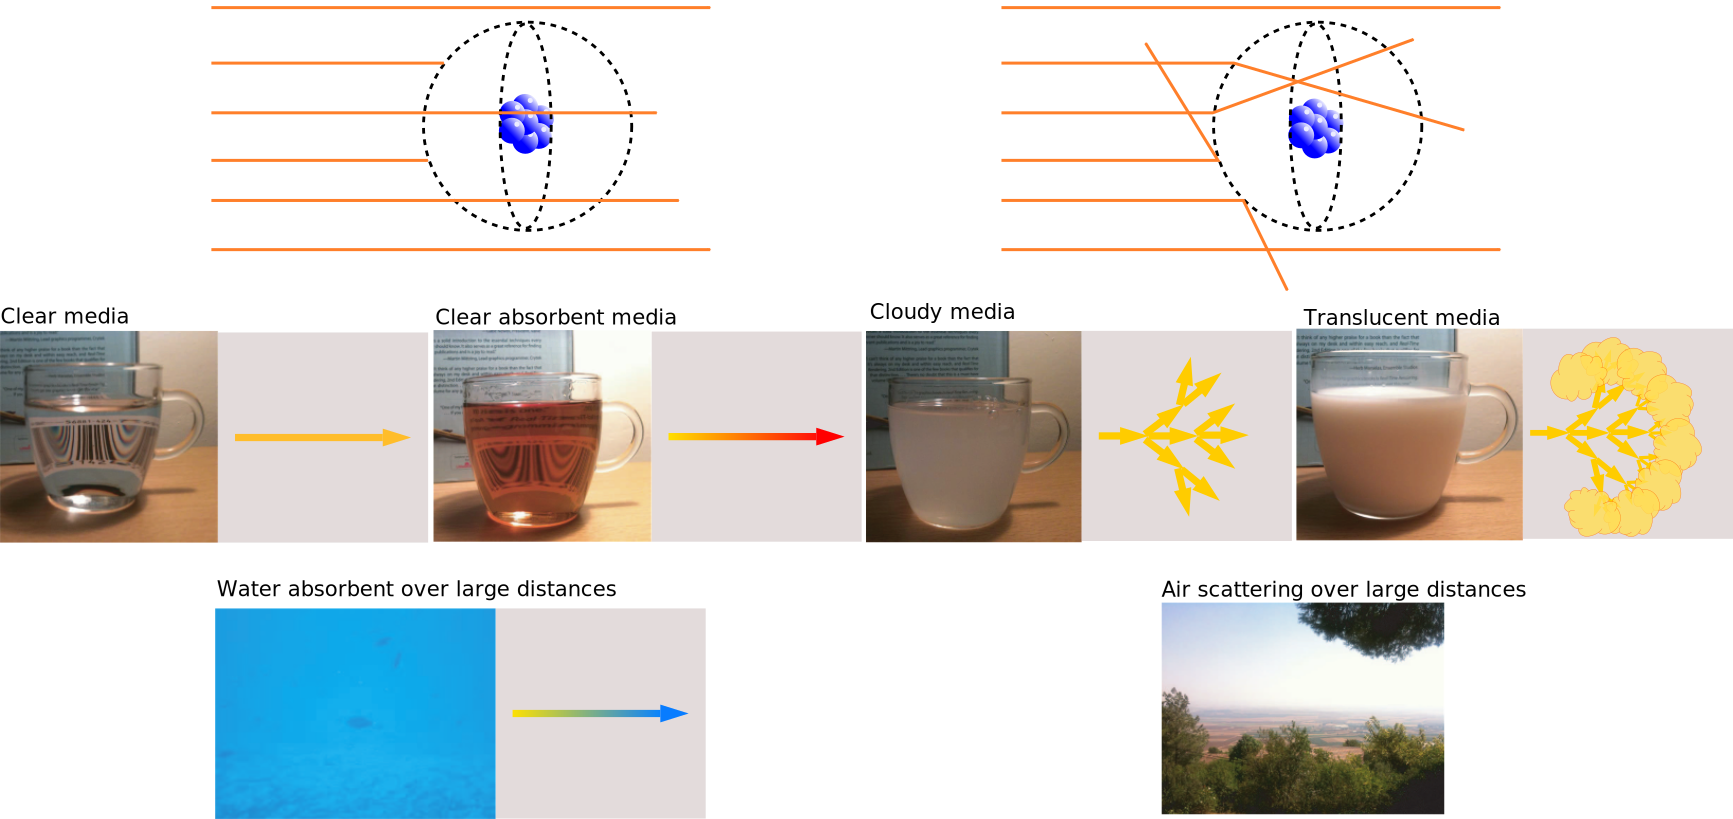
\includegraphics[width=\textwidth]{pics/physicallyBasedRendering/scattering_absorption2/scattering_absorption}
\end{frame}

\begin{frame}
    \frametitle{Absoption, scattering}
    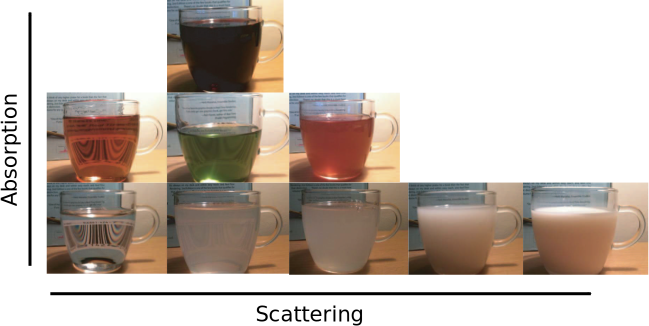
\includegraphics[width=\textwidth]{pics/physicallyBasedRendering/scattering_absorption1/scattering_absorption}
\end{frame}

\begin{frame}
    \frametitle{Specular, diffuse component}
    
\includegraphics[width=\textwidth]{pics/physicallyBasedRendering/specular_diffuse}
\end{frame}

\begin{frame}
    \frametitle{Subsurface scattering}
    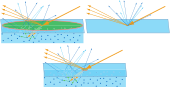
\includegraphics[width=\textwidth]{pics/physicallyBasedRendering/subsurface_pixel_size}
\end{frame}

\begin{frame}
    \frametitle{Lom světla kovů}
    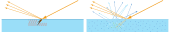
\includegraphics[width=\textwidth]{pics/physicallyBasedRendering/metal_refraction}
\end{frame}

\begin{frame}
    \frametitle{Drsnost povrchu a mikroplošky}
    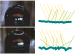
\includegraphics[width=\textwidth]{pics/physicallyBasedRendering/roughness/roughness.pdf}
\end{frame}

\begin{frame}
    \frametitle{Zastínění mikroplošek}
    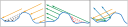
\includegraphics[width=\textwidth]{pics/physicallyBasedRendering/microfacets_occlusion}
\end{frame}

\begin{frame}
    \frametitle{Zastínění mikroplošek}
    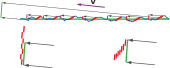
\includegraphics[width=\textwidth]{pics/physicallyBasedRendering/microfacet_masking}
\end{frame}



\begin{frame}
    \frametitle{State of the art}
    \includegraphics[width=\textwidth]{pics/physicallyBasedRendering/pbr}
    \pause\vfill
    Dneska jen kousek :(
\end{frame}

\begin{frame}
    \frametitle{Osvětlení}

    \begin{columns}[c]
    \column{.5\textwidth}

    \includegraphics[width=\textwidth]{pics/physicallyBasedRendering/bunny}

    \column{.5\textwidth}

    \includegraphics[width=\textwidth]{pics/physicallyBasedRendering/stanford-bunny}
    
    \end{columns}
\end{frame}

\begin{frame}
    \frametitle{Zobrazovací rovnice}
    \begin{equation*}
        L_o(\mathbf x, \omega, \lambda, t) = L_e(\mathbf x, \omega, \lambda, t) + \int\limits_\Omega f_r(\mathbf x, \omega', \omega, \lambda, t) L_i(\mathbf x, \omega', \lambda, t) (-\omega' \cdot \mathbf n) d \omega'
    \end{equation*}
    \includegraphics[width=2in]{pics/physicallyBasedRendering/rendering}
    \vfill
    Siggraph 1986 :
    \begin{equation*}
        \displaystyle I(x, x') = g(x, x')\left[ e(x, x') + \int\limits_S p(x, x', x'')I(x', x'')dx''\right]
    \end{equation*}
\end{frame}

\begin{frame}
    \frametitle{Lokální osvětlovací model}

    \begin{itemize}
        \item Odraz světla v "jednom bodu".
        \item Diferenciální ploška scény.
    \end{itemize}
    \pause\vfill
    \begin{equation*}
        L_{\{o,e,i\}}(\mathbf x, \omega, \lambda, t)
    \end{equation*}
    \begin{itemize}
         \item Radiance
         \item $W \cdot sr^{-1} \cdot m^{-2} (\cdot m^{-1})$
    \end{itemize}
    \pause\vfill
    \begin{equation*}
        f_r(\mathbf x, \omega', \omega, \lambda, t)
    \end{equation*}
    \begin{itemize}
        \item BRDF
        \item $sr^{-1}$
    \end{itemize}
\end{frame}

\begin{frame}
    \frametitle{BRDF}
    \begin{itemize}
        \item Bidirectional Reflectance Distribution Function.
        \item Hustota pravděpodobnosti (skoro).
    \end{itemize}
    \pause\vfill
    Reciprocita
    \begin{equation*}
        f_r(\mathbf x, \omega', \omega) = f_r(\mathbf x, \omega, \omega')
    \end{equation*}
    Zákon zachování energie
    \begin{equation*}
        \int\limits_\Omega f_r(\mathbf x, \omega', \omega) (\omega \cdot \mathbf n) d\omega \le 1
    \end{equation*}
    Izotropie x Anizotropie
\end{frame}

\begin{frame}
    \frametitle{Varianty BRDF}
    \begin{itemize}
        \item Phong
        \item Blinn-Phong
        \item Cook-Torrance
        \item GGX
        \item ...
    \end{itemize}
    \pause\vfill
    \begin{itemize}
        \item Pragmatické x Fyzikální
        \item Výběr podle aplikace.
    \end{itemize}
\end{frame}

\section{Odraz světla}

\begin{frame}
    \frametitle{Odraz a lom světla}
    \includegraphics[width=.4\textwidth]{pics/physicallyBasedRendering/image106}
    \begin{itemize}
        \item Odraz a lom na hranicích prostředí.
        \item Indexy lomu (rychlost v daném prostředí).
        \item Polarizace odrazem.
    \end{itemize}
    \begin{equation*}
        \frac{v_1}{v_2} = \frac{\sin\alpha}{\sin\beta}
    \end{equation*}
\end{frame}

\begin{frame}
    \frametitle{Energie}
    Fresnellovy vzorce
    \begin{equation*}
        R_s = \left| \frac{Z_2 \cos \theta_i - Z_1 \cos \theta_t}{Z_2 \cos \theta_i + Z_1 \cos \theta_t} \right|^2
    \end{equation*}
    \begin{itemize}
        \item Závislé na polarizaci.
        \item Nepraktické.
    \end{itemize}
    \pause\vfill
    Schlickova aproximace
    \begin{equation*}
        R(\theta) = R_0 + (1-R_0)(1-\cos\theta)^5
    \end{equation*}
    \begin{itemize}
        \item $R_0$ je vlastnost materiálu.
        \item Pro izolanty $R_0 \approx 0.04$.
        \item $\cos\theta \rightarrow 0$ ... $R \rightarrow 1$
    \end{itemize}
\end{frame}

\begin{frame}
    \frametitle{Fresnel reflectance}
    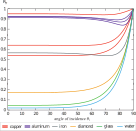
\includegraphics[width=0.8\textwidth]{pics/physicallyBasedRendering/fresnel_reflectance}
\end{frame}

\begin{frame}
    \frametitle{Fresnel reflectance}
    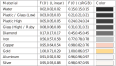
\includegraphics[width=\textwidth]{pics/physicallyBasedRendering/fresnel_reflectance_table}
\end{frame}

\begin{frame}
    \frametitle{Nedokonalý povrch}
    \includegraphics[width=\textwidth]{pics/physicallyBasedRendering/night-reflect}
\end{frame}

\begin{frame}
    \frametitle{Mikroploškový model}
    \includegraphics[width=.5\textwidth]{pics/physicallyBasedRendering/mf}
    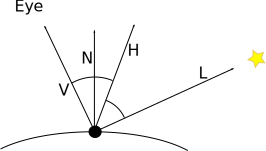
\includegraphics[width=.5\textwidth]{pics/physicallyBasedRendering/half}\\
    Které plošky jsou správně orientované?
    \pause
    \begin{itemize}
        \item Odrážejí ze světla do pozorovatele.
        \item Mají normálu přesně mezi.
        \item[!] Half vector.
    \end{itemize}
    \begin{equation*}
        \mathbf h = \frac{\mathbf l + \mathbf v}{2}
    \end{equation*}
\end{frame}

\begin{frame}
    \frametitle{Diffuse + Specular}
    \includegraphics[width=\textwidth]{pics/physicallyBasedRendering/ds} \\
    Specular
    \begin{itemize}
        \item "Zrcadlový" odraz
        \item Dominantní pro kovy
    \end{itemize}
    Diffuse
    \begin{itemize}
        \item Odraz uvnitř materiálu.
        \item Dominantní pro izolanty.
    \end{itemize}
\end{frame}

\begin{frame}
    \frametitle{Cook-Torrance}
    Spekulární odraz
    \begin{equation*}
        f_r(\mathbf x, \mathbf l, \mathbf v) = \frac{F(\mathbf l, \mathbf h)G(\mathbf l, \mathbf v, \mathbf h)D(\mathbf h)}{4(\mathbf n \cdot \mathbf l)(\mathbf n \cdot \mathbf v)}
    \end{equation*}
    \begin{itemize}
        \item F - Fresnell/Schlick
        \item D - Distribuční funkce plošek
        \item G - Geometrické zastínění plošek
    \end{itemize}
\end{frame}

\begin{frame}
    \frametitle{Blinn-Phong}
    \begin{equation*}
        D(\mathbf h) = (\mathbf n \cdot \mathbf h)^{\mathrm shininess}
    \end{equation*}
    \includegraphics[width=.5\textwidth]{pics/physicallyBasedRendering/shininessGraph}
    \includegraphics[width=.5\textwidth]{pics/physicallyBasedRendering/shininess.png}
\end{frame}

\begin{frame}
    \frametitle{Dohromady}
    \begin{equation*}
        f_r(\mathbf x, \mathbf l, \mathbf v) = (R_0 + (1-R_0)(1-(\mathbf l \cdot \mathbf h))^5)(\mathbf n \cdot \mathbf h)^{\mathrm shininess}
    \end{equation*}
    Co chybí?
    \begin{itemize}
        \item Barva materiálu (izolantú). $R_0$ je "barva kovu".
        \item[!] Lomené paprsky.
        \item Zachování energie.
    \end{itemize}
\end{frame}

\begin{frame}
    \frametitle{Difúzní odraz}
    \begin{equation*}
        f_r(\mathbf x, \mathbf l, \mathbf v) = \frac{k_d}{\pi}
    \end{equation*}
    \begin{itemize}
        \item Nezáleží na poloze pozorovatele.
        \item $1/\pi$ je zachování energie.
    \end{itemize}
    \begin{equation*}
        \int\limits_\Omega 1/\pi d\omega = 1
    \end{equation*}
\end{frame}

\begin{frame}
    \frametitle{Diffuse + Specular}
    \begin{equation*}
        \left(\frac{k_s}{\pi} + k_n(R_0 + (1-R_0)(1-(\mathbf l \cdot \mathbf h))^5)(\mathbf n \cdot \mathbf h)^{\mathrm shininess}\right)(\mathbf n \cdot \mathbf l)
    \end{equation*}
    \begin{equation*}
        k_n = \frac{(\mathrm shininess + 2)(\mathrm shininess + 4)}{8\pi(2^{-\frac{shininess}{2}} + shininess)}
    \end{equation*}
    \begin{itemize}
        \item $\mathbf n \cdot \mathbf l$ z renderovací rovnice.
        \item Zachování energie pro specular.
        \item Odvození na \url{http://www.farbrausch.de/~fg/stuff/phong.pdf}
    \end{itemize}
\end{frame}

\section{Bodový zdroj světla}

\begin{frame}
    \frametitle{Bodový zdroj světla}
    \begin{equation*}
        L_o(\mathbf x, \omega, \lambda, t) = L_e(\mathbf x, \omega, \lambda, t) + \int\limits_\Omega f_r(\mathbf x, \omega', \omega, \lambda, t) L_i(\mathbf x, \omega', \lambda, t) (-\omega' \cdot \mathbf n) d \omega'
    \end{equation*}
    \begin{itemize}
        \item Bod má nulovou plochu.
        \item Bodové zdroje jsou singularity.
        \item Jak upravit renderovací rovnici? Jaké $L_i$?
        \pause
        \item Nastavíme ho přes barvu ideálního difúzního povrchu.
    \end{itemize}
    \begin{align*}
        L_o &= \int\limits_\Omega \frac{1}{\pi} L_i (-\omega' \cdot \mathbf n) d \omega' \\
        L_i &= \pi L_o
    \end{align*}
\end{frame}

\begin{frame}
    \frametitle{Pohromadě}
    \begin{equation*}
        L = \sum_i \left(\frac{k_s}{\pi} + k_n F(R_0, \mathbf l_i,\mathbf h_i)(\mathbf n \cdot \mathbf h_i)^{\mathrm shininess}\right)(\mathbf n \cdot \mathbf l_i) \pi L_i
    \end{equation*}
    \begin{itemize}
        \item Sčítáme přes světla.
        \item $\pi$ se vykrátí.
    \end{itemize}
    \pause
    \vfill
    Co tam chybí?
    \pause
    \begin{itemize}
        \item Vzdálenost od světla $L_i = f(|\mathbf p_i - \mathbf x|^2)$
        \item Světelný kužel.
        \item Vícenásobný odraz světla.
    \end{itemize}
\end{frame}

\begin{frame}
    \frametitle{Ambientní světlo}
    \begin{align*}
        L_o &= \sum_i k_a L_i \\
        k_a &= k_d 
    \end{align*}
    \vfill
    \includegraphics[width=2.5in]{pics/physicallyBasedRendering/ambient}
    \begin{itemize}
        \item Hrubá aproximace mnohonásobného odrazu světla.
    \end{itemize}
\end{frame}

\section{Normály}

\begin{frame}
    \frametitle{Normálové vektory}

    \begin{itemize}
        \item Kolmé k povrchu
        \item $\left| N \right| = 1$ (normalizované)
        \item 1 na trojúhelník/1 na vrchol
        \vfill
        \item $\displaystyle \vec{N_{\mathrm{face}}} = \vec{AB} \times \vec{AC}$
        \item $\displaystyle \vec{N_{\mathrm{vertex}}} = \mathrm{normalize}\left( \sum\limits_{i=1}^n N_{\mathrm{face}i} \right)$
        \item Prúměr vážený plochou trojúhelníkú
        \vfill
        \item Transformace :
        \begin{itemize}
            \item Rotace \emph{+ posun} - $N_{\mathrm{eye}} = ModelView \cdot N_{\mathrm{model}}$
            \item Scale - $N_{\mathrm{eye}} = (ModelView^T)^{-1} \cdot N_{\mathrm{model}}$
            \item[\color{red}!] Při scale je nutné vektory po transformaci znovu normalizovat!
        \end{itemize}
    \end{itemize}
\end{frame}

\begin{frame}
    \frametitle{Stínování}

    "Flat" stínování
    \begin{itemize}
        \item Osvětlují se celé trojúhelníky.
        \item Nic se neinterpoluje.
    \end{itemize}

    Gouraudovo stínování - "per vertex lighting"
    \begin{itemize}
        \item Osvětlení se počítá pro vrcholy.
        \item Interpolují se barvy.
        \item Dnes už nemá smysl.
    \end{itemize}

    Phongovo stínování - "per fragment lighting"
    \begin{itemize}
        \item Osvětlení se počítá pro fragmenty.
        \item Interpolují se normálové vektory.
    \end{itemize}

    \includegraphics[width=\textwidth]{pics/physicallyBasedRendering/shading}
\end{frame}

